\documentclass[12pt]{report}
\usepackage[english]{babel}
\usepackage[utf8x]{inputenc}
\usepackage{graphicx}
\usepackage{amsmath}
\usepackage[colorinlistoftodos]{todonotes}
\usepackage{float}
\usepackage[T1]{fontenc}
\usepackage{subfigure}
\usepackage{algorithmic}
\usepackage{algorithm}
\usepackage{color}
\usepackage{pdfpages}
\usepackage{microtype}
\usepackage{enumitem}
\usepackage{setspace}
\usepackage[left=2cm, right=2cm, top=2cm]{geometry}
\usepackage[toc,page]{appendix}
% % % % % % % % % % % % % % % % % % % % % %
\begin{document}
% % % % % %Front Page % % % % % % % % % % %
\begin{titlepage}
\center

\textsc{\large Seminar Report On}\\[1.0cm] % Name of your university/college
\textsc{\Large BLOCKCHAIN IN HEALTHCARE DOMAIN}\\[1.0cm] % Major heading such as course name
\textsc{\large Submitted in Partial Fulfillment of the Requirements for the award of \\ Bachelor of Technology in \\ Computer Science and Engineering\\ (2015-2019)}\\[0.5cm] 

\begin{figure}[H]
\centering

\includegraphics[width=0.7\textwidth]{logo.png}\\
%\label{logo}
\end{figure}

\vspace{2.0cm}
\begin{minipage}{0.4\textwidth}
%\begin{flushleft} 

\center
\
\large
\emph{Submitted By:}\\
\hspace{0.0cm}Basil K Y\\
\hspace{0.0cm}Reg No. MUT15CS019\\
%\end{flushleft}
\end{minipage}\\[2cm]
~~~~~~~~~~~~~~~~~~~~


\textbf{Department of Computer Science and Engineering}\\
\textbf{Muthoot Institute of Technology and Science (MITS)} \\
Varikoli P.O, Puthencruz-682308
\end{titlepage}
% % % % % % % % % % % % % % % % % % % % % % % % %
\newpage\begin{titlepage}
\center


\textsc{ \textbf{MUTHOOT INSTITUTE OF TECHNOLOGY \& SCIENCE}}\\
\textsc{\textbf{Varikoli P.O, Puthencruz-682308}}
\vspace{0.7cm}
\begin{figure}[H]
\centering

\includegraphics[width=0.7\textwidth]{logo.png}\\
%\label{logo}
\end{figure}
\vspace{0.2cm}
\textsc{ \small \textbf{ DEPARTMENT OF COMPUTER SCIENCE \& ENGINEERING}}\\
\section*{\centering CERTIFICATE}
%\thispagestyle{empty}
\begin{center}
 This is to certify that the seminar report entitled \textbf{"BLOCKCHAIN IN HEALTHCARE DOMAIN"} submitted by \textbf{Basil K Y (MUT15CS019)} of Semester VII is  a bonafide account of the work done by him under our supervision\\
\end{center}
\vspace{5cm}




\noindent  \emph{Guide} \hspace{3.6cm} \emph{Coordinator}\hfill \emph{Head of the Department}
\\
\noindent Mr. Bineeth Kuriakose\hspace{0.82cm}Ms Rakhee M \hfill Dr. Anand Hareendran S\\
\noindent Asst. Professor\hspace{2.10cm} Asst. Professor\hfill Asso. Professor\\
\noindent Dept. of CSE\hspace{2.39cm} Dept. of CSE\hfill Dept. of CSE
%\noindent\textbox{Left longer sample text\hfill}\textbox{\hfil Center\hfil}\textbox{\hfill Right




\end{titlepage}
\newpage
\pagenumbering{roman}

\section*{\centering Acknowledgements}
\vspace{1cm}
\par This seminar is the result of my hard work wherein I have been helped and supported by several persons and institutions directly and indirectly. Now it is the time to acknowledge their contributions. 

\par First of all to the Great Almighty, the author of knowledge and wisdom for his countless love.I would like to sincerely thank my guide \textbf{Asst. Prof. Bineeth Kuriakose}, for his support and valuable guidance.With great respect, I express my sincere thanks to our Head of The Department \textbf{Dr. Anand Hareendran} for all the proper guidance and encouragement. I extent my gratitude to the seminar coordinators \textbf{Asst. Prof.Rakhee M}, \textbf{Prof. Dr. Raju.C.K} and \textbf{Asst. Prof. Resmi.N.G} for their timely advice, meticulous scrutiny, scholarly advice and scientific approach that helped to a very great extent throughout the seminar.

\par I express my heartfelt veneration to all who had been helpful and inspiring throughout this endeavour.

\vspace{1cm}
\null\hfill \textbf{Basil K Y}
\newpage

\begin{abstract}

Blockchain is an emerging technology with tremendous applications in various sectors including healthcare. A number of blockchain based solutions and concepts have been emerged to solve or to find enhanced solutions for existing problems in healthcare sector. Many multinational companies are also confident in investing in blockchain based solutions over healthcare. The decentralized peer to peer networking of blockchain can ensure trust between participating entities in the network. Even though there are different opinions on how to apply blockchain technology, they seems to be promising to find potential solutions. Blockchain technology have a couple of use cases in healthcare including supply chain management,drug authenticity validation,clinical trials,claim adjudication etc. Even though there are numerous advantages for applying blockchain, there are big challenges existing including uncertainty,storage capabilities,scalability,cost etc. These challenges have to be overcome inorder to find solutions for problems in healthcare for a better tomorrow.
\end{abstract}

\tableofcontents
\addcontentsline{toc}{chapter}{List of Figures}

\listoffigures
%\addcontentsline{toc}{chapter}{List of Tables}
%\listoftables

% % % % % % % %% % % % % % % % % % % % % % % % % %

\chapter{Introduction}
\par
Blockchain is a distributed and decentralized chain of records or ledgers.
The immutability of blockchain records ensures trust between participating entities.
At its core, blockchain is a distributed system for recording and storing transaction
records.
More specifically, blockchain is a
shared, immutable record of peer to peer
transactions built from linked transaction
blocks and stored in a digital ledger.
Blockchain relies on established
cryptographic techniques to allow each
participant in a network to interact (e.g.
store, exchange, and view information),
without preexisting trust between the
parties. In a blockchain system, there is no
central authority; instead, transaction
records are stored and distributed across all
network participants. Interactions with the
blockchain become known to all participants
and require verification by the network
before information is added, enabling
trustless collaboration between network
participants while recording an immutable
audit trail of all interactions.This has lead to a wide range of applications for blockchain on different domains like banking,financial transactions,social media platforms,crypto currencies etc.The impact of blockchain technology can also be seen in the healthcare industry also. Technologists and healthcare providers and professionals across the globe view blockchain technology as a crucial way to implement the sharing of medical records in a secure way to protect patient's personal data from outsiders, and give patients more control over their information.Various blockchain based solutions have been emerged to enhance current situation of healthcare.
\pagenumbering{arabic}

\chapter{Problems in Healthcare Sector}

The current healthcare infrastructure has often been called inadequate to handle information exchange and requires certain tweaks.Health record sharing in current scenario doesn't take care about the privacy of patients and patients have less control over their own data.The following is a list of main problems healthcare industry and the patients faces today.
\section{Interoperability of Healthcare Data}
\frenchspacing
Currently, there is no accepted standard for the sharing of health data from one hospital to another.Most of the cases, patient has to carry all of his past medical records to the new hospital or have to do the previous medical tests again.It’s difficult to simply copy information from one piece of EHR software to another. Mismatched types, strange data fields, and proprietary formats mean that data has to be manipulated and sanitized before it can be imported into another system. This lack of a common standard for capturing, transmitting, receiving, storing, and managing patient data causes delays and inaccuracies.Some EHR and healthcare system vendors are holding patient data for ransom. They charge fees for transmitting data outside the system, increasing operational costs and making providers less likely to send data to others in the healthcare supply chain. The government is acting to encourage interoperability, but not all vendors have taken this on board.There is no way to consistently identify a patient across multiple systems or providers. Patients can give their name, date of birth, and other identifying data, but because different systems store this information in different ways, errors are possible. There is a push towards a unique patient identifier, a code that could be used to categorically identify the same individual no matter what system or provider they used. Unfortunately, we are still far from getting this most basic of functionalities in place.There is also a lack of standards for sending, receiving, and managing information between EHR systems.

\section{Fragmented Patient Records}
\par Patient data is scattered across many hospitals and healthcare service  providers. Patient doesn't have a longitudinal list of their past health records. Duplication of health records can occur within hospitals also. Different records may be generated for same patient if he forgets his unique IDs.Many hospitals in rural areas are still following physical records which makes the record handling even complex.The records are more prone to tampering and loss.
Patients regularly encounter fragmented systems of care and the results often lead to unmet social needs, conflicting medications, incorrect dosages etc. Many of patients that are the most affected by fragmented care coordination are populations that are already at risk for chronic illnesses and have an array of unmet social needs.
\section{Claim Adjudication}
Current existing patient billing management systems are at best complex and prone to manipulation by the service providers.Today, an estimated 50\% of healthcare costs are fraudulent, resulting from excessive
billing or billing for non performed services.Also Currently, 22\% of claims get rejected either because they are not received by the insurer or they contain defects, such as incomplete or incorrect demographic
data or lack of proof supporting the services billed\cite{7}.There is a lack of trust between participants in the healthcare industry as medical records are easily changed by hospitals or patients for getting health insurances.It is easy to tamper the data if it is stored centrally at a place.So,it is important to ensure that all
claims submitted for payment are coded accurately.
\section{Data Privacy and Security}
Since patient doesn't has the full control over his data, third parties can easily misuse the data.There are currently no mechanism available to share data in a permissioned and time bound manner.Sensitive data in healthcare can include patient data like protected health information, stored data such as medical and payment records, medical devices data etc. which are ubiquitous in healthcare environments.But healthcare organizations are not always properly prepared for managing and protecting their big data. That’s because IT departments within healthcare organizations often lack the budget necessary to bolster big data security.Data breaches, like the one that exposed nearly 38 million Anthem Health Insurance patient records, are becoming increasingly common. The healthcare industry has the highest risk factor when it comes to experiencing a data breach. Statistics show 88\% of all ransomware attacks in 2017 targeted the healthcare industry.\cite{12}.Healthcare records are considered highly valuable to cyber attackers. This is because of the richness of personal, medical, financial information contained within each EHR. Data thieves can easily resell this information on the dark web. With access to this information, identity theft, insurance fraud, and financial fraud is committed for financial gain by criminal elements.But data is at risk even if an organization does not suffer an outside attack. Information can be leaked internally when employees, contractors, and IT security personnel do not take the proper precautions to manage and protect their data.

\section{Ill-informed Clinical Decision
Making \cite{3}}Traditionally, an investigation or test should only be requested and arranged if this is going
to lead to a different possible
diagnosis or alternative treatment Unfortunately, even when
test have returned, these are
rarely shared widely with all of
the health professionals involved
in the patient’s care and are
normally isolated, at the
institution which requested them
originally.
The patient’s quality of care
suffers as a result of this. Other
institutions are not aware of a
patient’s complete history and in
turn, this could lead to incorrect
decision making, delays, and
unnecessary costs for the patient
or health institution. In the worst
case, these medical errors can be
fatal.

\section{Data Reliability}
Health data of patients should be instantly accessible when there is a need, to provide proper treatment on time.Most of the service providers are storing health data locally in their database.This causes high potential for data reliability and data loss.If the system fails, entire patient health records gets destroyed.Cloud based duplication of data is necessary to reliably store data loss.

\section{Lack of Transparency}
The entire system is not patient centric and patient doesn't have full control over his/her data.Since patient doesn't have control over their data, what happen with their data is hidden to the patient.Hospitals or service providers may sell patient's data to third parties without their permission.

\chapter{Blockchain Applications in Healthcare}
\par The Blockchain is the leading technology which actually took the world by storm by its revolutionary work in data management and exchange, specifically in the financial sector. Its huge success in different industries has actually made healthcare world come up with questions too. People are explaining it as the answer to inter-operability and healthcare’s looming problems but if the confusion looms then the Blockchain will take far more time to bring the difference in the healthcare sector.Health data  need to be stored securely and privacy of patients needs to be considered when sharing data.Thre are lots of areas within healthcare where blockchain can be applied. Blockchain can provide patient centric longitudinal health records, supply chain management, claim adjudication, drug verification, permissioned data sharing and a lot more. There are existing solutions and implementation concepts available. The following are the main use cases of blockchain in  healthcare, together with how it is implemented in different healthcare services.
\begin{figure}[H]
\centering
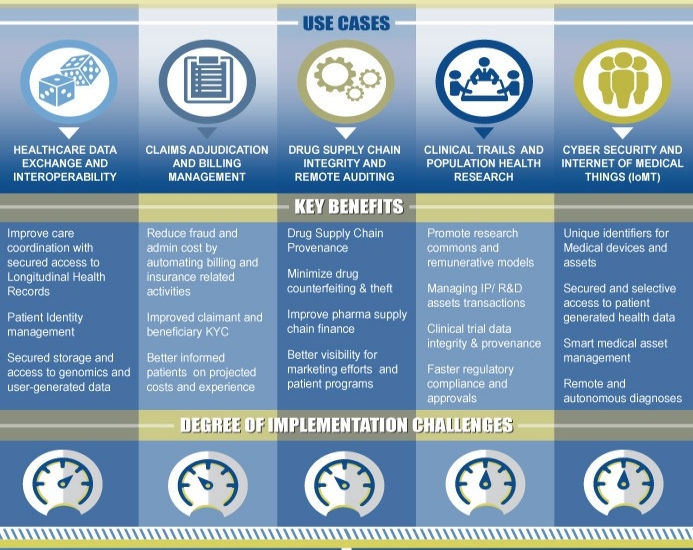
\includegraphics[width=0.9\textwidth]{apps.jpg}
\caption{Blockchain use cases in healthcare \cite{13}}
\label{usecase}
\end{figure}
\section{Personal Health Records}
The architecture of blockchain is like a series of immutable records.This is highly helpful in implementing a patient centric chain of health records.The series of health records of patients can be linked on the basis of time as patient goes for different services at different providers.The following are the different concepts on how to implement this longitudinal list of records.
\subsection{Medrec \cite{2}}
In Medrec, the longitudinal ist of records are implemented using Summery Contracts(SC).This is a special kind of etherium contract which functions as a bread crumb trail for participants in the system to locate their medical record history.It holds a list of references to Patient Provider Relationship contracts (PPRs).A Patient Provider Contract is issued when a service provider like hospital adds health records for a patient.Thus SC represents all the patient's previous and current engagements with other service providers in the system. Providers can also have SC with references to patients for whom they have given services. SC can be used to provide backups, notifications,granting and revoking access permissions etc.
\begin{figure}[H]
\centering
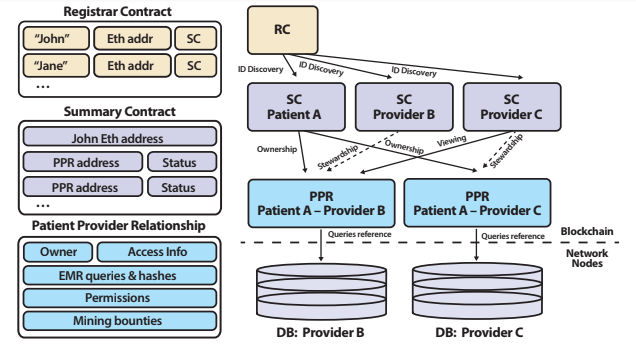
\includegraphics[width=0.9\textwidth]{ppr.png}
\caption{Summery Contract and PPR}
\label{ppr}
\end{figure}
\section{Health Information Exchange}
Currently, the healthcare industry experiences major inefficiencies due to diverse and unconnected data. Effective care collaboration is vital to improve healthcare outcomes. With digitized health data, the exchange of healthcare information across healthcare organizations is required.Data sharing should be done only by considering privacy of patients.The push for nationwide interoperability and improved health data exchange have increased records sharing, which can create advantages and difficulties for providers.
\par One of the major challenges, is the lack of a universal identifier.Two systems may  not automatically able to identify the patient because she was registered under a different name in each system.A common understanding between service providers is needed to resolve this.Patient authorization and consent is often cited as one of the first challenges to share medical data, because authorization is a true test of the ability of EMR systems to work across healthcare and technology platforms as data is exchanged.Competition among providers is also creates hindrance for sharing medical data. Organizations will continue to compete for patients, but they will not compete on sharing information.Different healthcare providers may have different strategies/standards to store and share healthcare data.It is hard for them to reach in a common agreement on how data should be represented for sharing.The additional cost involved in developing the sharing mechanism is a burden for service providers.This additional cost involved make it impossible for small developing firms to compete with big players.

\begin{figure}[H]
\centering
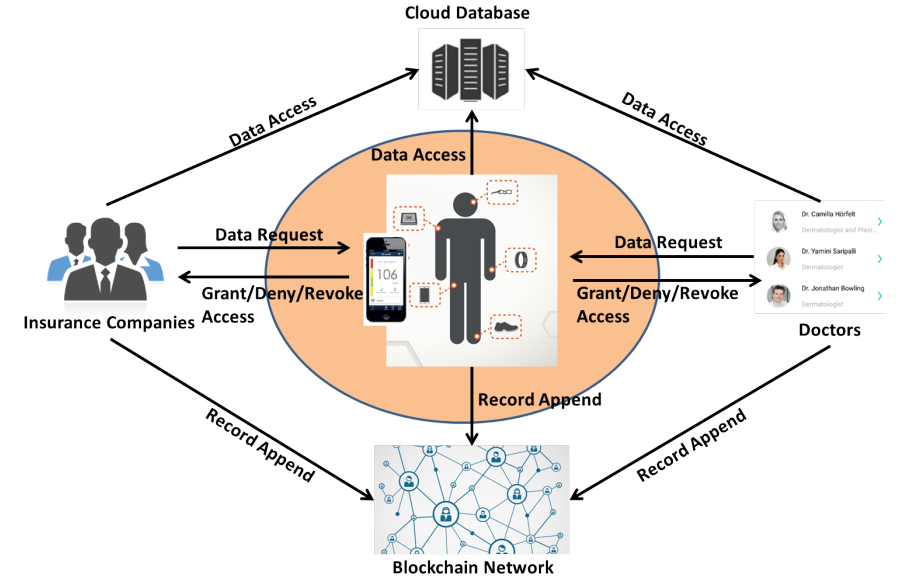
\includegraphics[width=0.9\textwidth]{centric.png}
\caption{Person centric data sharing \cite{13}}
\label{centric}
\end{figure}
\subsection{Medrec}
\par A Patient-Provider Relationship Contract is issued between two nodes in the system when one node stores and manages medical records for the other(eg:hospital and a patient). The PPR defines an assortment of data
pointers and associated access permissions that identify the records held by the care provider. Each pointer
consists of a query string that, when executed on the provider's database, returns a subset of patient data.
The query string is affixed with the hash of this data subset, to guarantee that data have not been altered
at the source. Additional information indicates where the provider's database can be accessed in the
network, i.e. hostname and port in a standard network topology. The data queries and their associated
information are crafted by the care provider and modified when new records are added. To enable patients
to share records with others, a dictionary implementation (hash table) maps viewers’ addresses to a list of
additional query strings. Each string can specify a portion of the patient's data to which the third party
viewer is allowed access. This can make things complex as an intermediate mechanism is needed to convert the queries to compatible types in the internal implementation at each hospitals.
\subsection{Medicalchain \cite{11}}
Any interactions with health records are recorded as transactions on the network.
Transactions are viewable only to the participants associated with the transaction.Medicalchain follows following procedures for information sharing.
\begin{description}
\item[$\bullet$] Patient A grants access to EHR to Practitioner A
\item[$\bullet$] Practitioner A’s ID is added to Patient A’s authorised asset on the ledger
\item[$\bullet$] Patient A’s ID is added to Practitioner A’s authorised asset on the ledger
\item[$\bullet$] The Symmetric key for the EHR is decrypted with Patient A’s private key
\item[$\bullet$] Symmetric key is then encrypted with Practitioner A’s public key
\end{description}
Similar kind of operations are done for revoking access.
\begin{figure}[H]
\centering
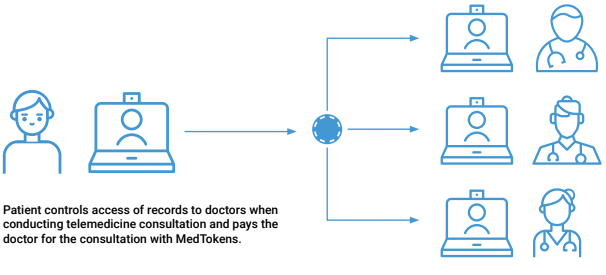
\includegraphics[width=0.9\textwidth]{sharing.png}
\caption{Sharing of Health Records}
\label{sharing}
\end{figure}

\subsection{Deloitte \cite{1}}
Deloitte uses patients private key to share their health data.Patients private key links their identity to blockchain data.Only organizations with this key can access the information and others can not.This have a potential risk as since private key is getting shared, the organizations can access the data for any period of time.Also, patient cannot selectively share data.As a transaction layer, the blockchain can
store two types of information: (1)
“On-chain” data that is directly stored on the
blockchain or (2) “Off-chain” data with links
stored on the blockchain that act as pointers
to information stored in separate, traditional
databases. Storing medical information
directly on the blockchain ensures that the
information is fully secured by the
blockchain’s properties and is immediately
viewable to those permissioned to access
the chain; at the same time, storing large
data files slows block processing speeds and
presents potential challenges to scaling the
system.
\begin{figure}[H]
\centering
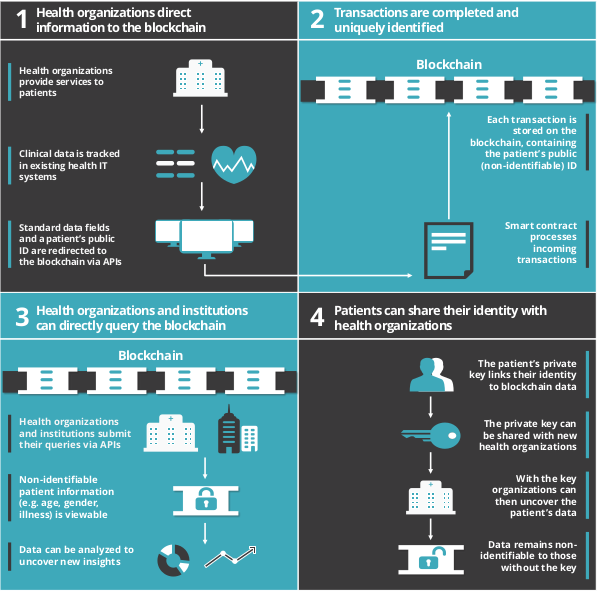
\includegraphics[width=0.9\textwidth]{diloitte.png}
\caption{Deloitte Implementation}
\label{diloitte}
\end{figure}

\section{Verifying the Authenticity of Drugs}

In the Pharma industry, drugs are frequently returned to the pharmaceutical manufacturers. For instance, wholesalers may have ordered excess inventory and accordingly may need to return unsold stock to the pharmaceutical manufactures.While the proportion of the returned drugs is small compared to the sales (about 2–3\% of sales), the per year volume is in the range of \$7- 10 billion\cite{14}.
Instead of destroying these perfectly good drug shipments, pharmaceutical companies instead opt to resell them. However before they can resell these returned drugs, the pharmaceutical companies have a legal obligation to verify the authenticity of the returned drugs(eg: Falsified Medicine Directive (FMD)).A far better and recommended approach is to have pharmaceutical manufacturers record the serial numbers of their packages on a blockchain, which serves as a decentralized and distributed ledger. Wholesalers and customers can then verify the authenticity of a drug package by connecting to the blockchain.
\begin{figure}[H]
\centering
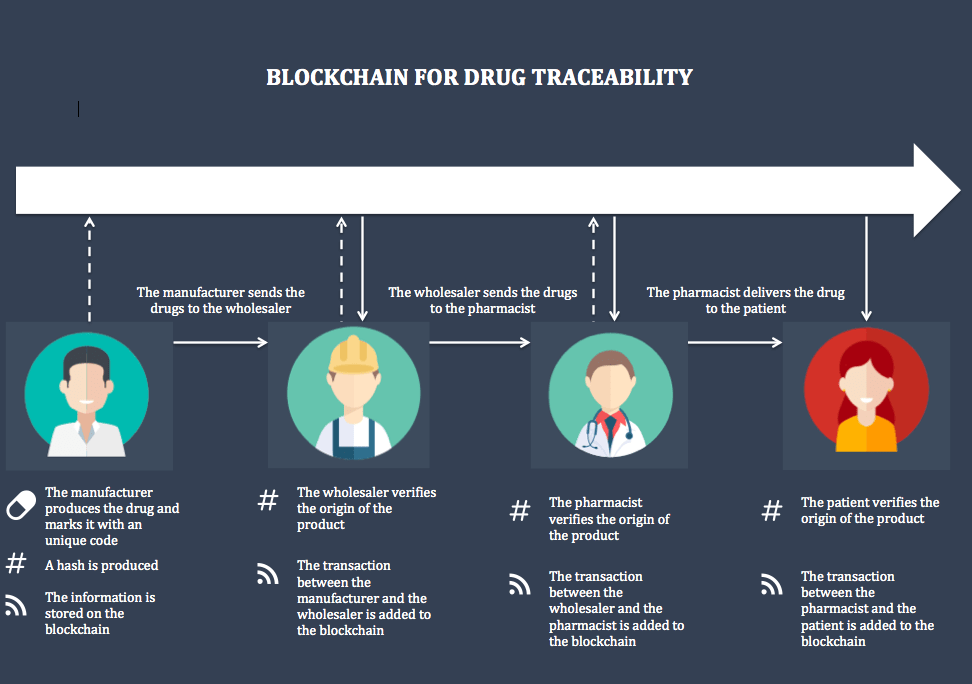
\includegraphics[width=0.9\textwidth]{drug.png}
\caption{ Verifying the Authenticity of Drugs}
\label{drug}
\end{figure}


\subsection{ATTP (Advanced Track and Trace for Pharmaceuticals) by SAP \cite{15}}
Merck in partnership with SAP has developed the SAP Pharma Blockchain POC app. SAP launched this first Proof of Concept in Q3 2017, and an improved version in early 2018.
\begin{description}
\item[$\bullet$]SAP’s existing solution (unrelated to blockchain) generates unique identifiers for a drug package.
\item[$\bullet$]When a manufacturer ships a package they register the item on the SAP Pharma POC blockchain, with the four pieces of information generated; the item number (based on GS1 standard), a serial number, a batch number, and an expiration date.
\item[$\bullet$]The distributor can extract the four pieces information from the packaging’s barcode, using a simple scanner mobile app, allowing them to verify returns .
\item[$\bullet$]Counterfeiter copies of barcodes can be avoided, since SAP has the added ability to track every time a package changes hands. A map view within the mobile app also helps ensure that the drugs are in the expected geographical region.
\end{description}
\section{Supply Chain Management}
Blockchain’s ability to track back to the origin of data makes it especially suited for this supply chain use case.The problem of counterfeiting is not just limited to drug manufactures, but extends to medical instruments manufactures. The World Health Organization (WHO) estimates that 8 percent of the medical devices in circulation today are counterfeit copies.Counterfeit drugs and medical devices pose a major risk to consumers, and also lost revenue for the legitimate manufacturers.
\subsection{Farmatrust \cite{16}}
is developing a platform based on blockchain technology to improve drug supply chain integrity. It is mainly focused on eliminating of counterfeit drugs proliferation and increasing efficiency in the pharmaceutical industry. The platform offers possibility to track pharmaceuticals through a supply chain that links digital systems to pharmaceuticals moving in the physical world. With a unique ID combined to a digital supply chain the FarmaTrust solution based on blockchain aims to eliminate proliferation of counterfeit drugs.
 
The platform will create a network of pharmaceutical brands, contract manufacturers and suppliers, logistics and shipping companies, wholesalers and distributors as well as pharmacies and hospitals. This network will then become a trusted system to ensure that medicines and related products are indeed the genuine product.
\begin{figure}[H]
\centering
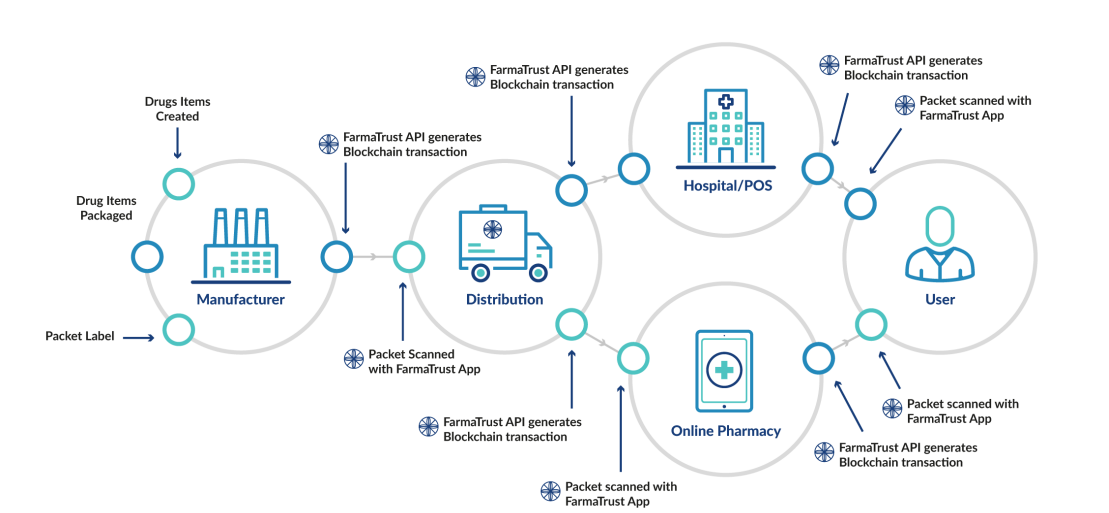
\includegraphics[width=1.0\textwidth]{farma.png}
\caption{Farmatrust Working}
\label{farmatrust}
\end{figure}


\section{Health Insurance Claim Adjudication}
\par The insurer may decide to pay the claim in full, deny the claim, or reduce the amount
paid to the provider. The decision to reduce a payment to the provider is typically made when
the insurance company has determined that the billed service is inappropriate or medically
unnecessary for the diagnosis or procedure codes. Therefore, it is important to ensure that all
claims submitted for payment are coded accurately. As soon as an insurance company receives a medical claim, they begin a thorough review. Sometimes even small errors such as a misspelled patient name may cause a claim to be rejected. The majority of claims today
are processed automatically without manual intervention, but as claims become more complex and are plagued by error and fraud, claim adjudication remains a challenging process.Fortunately, smart contracts present
an opportunity for automating the adjudication process further by distributing and thus making claims transparent to the provider and insurer, exposing potential errors and frauds that
can be corrected or investigated in a much timelier manner. Another benefit of creating these
pre-established agreements via smart contracts is to ensure involved participants are up to date and properly notified as policies or rules change.
Smart contracts present
an opportunity for automating the adjudication process further by distributing and thus making claims transparent to the provider and insurer, exposing potential errors and frauds that
can be corrected or investigated in a much timelier manner.

\section{Patient Digital Identity}
\par Without common standards for collecting patient identifying information, even the
same patient’s identity can vary from one care facility to another.  Furthermore, patient information manually
entered into the system may contain typos or errors, and the more data collected, the more
opportunities for mistakes. Although within each organization patient demographics data
may be collapsed into a single unique ID, the ID generally does not translate across organizations.
Without a functional, unified identity management system, patient identification
schemes employed at various care sites may continuously experience incompatibility and patient matching problems, unless a patient exclusively receives care within one organization.
\par
The very nature of Blockchain incorporates such a decentralized, unified identity system. Many existing Blockchains use cryptographically secured addresses to represent identities. Each address is mathematically linked with a unique key that is used to easily verify theownership of an address or an identity yet does not reveal any personal information relating
to the individual. The decentralized and auditable characteristics of Blockchain can help enforce standardized verifiable identities for patients via a universal patient index registry sharable across all healthcare facilitates within a nation and beyond. In case of lost or stolen keys, new addresses are also trivial to generate and reassign to patients.

\section{Clinical Trials}
In the pharmaceutical industry, clinical trials are designed to test the tolerance and effectiveness of a product on a group of patients in order to validate or invalidate hypothesises. Usually they take several years and the outcomes are critical for the future of the drug.During clinical trials, a considerable amount of data is produced safety and quality reports, statistics, blood tests, surveys, medical imagery and large groups of people are involved, making it hard to track and control everyone\cite{17}. Hence, mistakes can be committed along the way, some unintentionally and others not.Fraud usually includes modifying or hiding data that could compromise the advance of the clinical trial and damage the image of an organization among regulatory agencies or patients. Different types of data can me modified or manipulated.
\par Fraud usually includes modifying or hiding data that could compromise the advance of the clinical trial and damage the image of an organization among regulatory agencies or patients. Different types of data can me modified or manipulated.The public key proves that a certain document was registered on the blockchain at a certain time. If during the trial, someone has doubts about the authenticity of data they encounter, they can verify that information they have is similar to the original information stored on the blockchain.

\section{Provider Directory \cite{14}}
\par Healthcare organizations, including payers, must maintain directories of healthcare providers, or doctors. Today this is done redundantly across multiple organizations. Further, if these directories get out of sync, it can lead to issues such as claims bouncing. Through blockchains, provider directories can be maintained by various healthcare organizations in a shared, decentralized ledger. This reduces redundancies and inconsistencies, and thereby improves operational efficiencies (including around claims adjudication).




\chapter{Advantages of using blockchain}
Blockchain's inherent transparent behaviour can ensure trust between parcipating agents.Instead of creating a new trusted “middle man” that mediates the establishment of
trust relationships between providers/hospitals, Blockchain technology offers the opportunity
for building trust.

\begin{description}
\item[$\bullet$]Ensures trust between participating entities.
\item[$\bullet$]Privacy and security for patients health data.
\item[$\bullet$]Data reliability.
\item[$\bullet$]Improved tracability of records.
\item[$\bullet$]Faster transaction rates.
\end{description}

\chapter{Challenges in Implementation}
Even though there are good reasons behind applying blockchain on healthcare sector,as of now, there are no well established EHR management platform based on blockchain which actually works.There are services under development including Medicalchain,Medrec etc.Big multinational companies like IBM are also investing in blockchain.

\subsection{Uncertainty}
The Blockchain concept is not widespread yet and there are only a few successful initiatives based on this modern technology at this time. That is a major hurdle because we don’t have many successful blockchain models to follow which creates an uncertain situation.
\subsection{Storage Capability}
\par Blockchain within the healthcare industry will be comprised of medical records, images, documents and lab reports which require a significant amount of storage space.Not only is it costly to store these data,but data access operations may also fail when the cost exceeds Blockchain network defined
data size limit.
\subsection{Scalability Challenge}
Providers, hospitals, insurance companies, and even departments within the same health organizations experience disconnectedness
caused by delays or the lack of information flow. Patients are commonly cared for at various
sources, such as private clinics, regional urgent care centers, enterprise hospitals, and telemedicine practice. A provider may serve hundreds or more patients whose associated health
activities must be tracked. Without any activity monitoring or filtering mechanism implemented, it would require tremendous computational effort for a provider to review a patient’s
health transactions on-demand.
\subsection{Adoption and Standardization}
Standardization of technical procedures on blockchain platforms in healthcare is cited to be the highest barrier to adoption by companies.
\subsection{Cost of Implemetation}
The cost of establishing and maintaining a healthcare blockchain is unknown yet and no one can seriously consider this technology without knowing about its expenses ahead of time.
\subsection{Rules and Regulations}
There are no rules available to address the use of blockchain in the healthcare industry. It is also uncertain as to how new policies regarding healthcare blockchain will conform to current privacy regulations like the HIPAA act.[18]

\subsection{Limited Performance \cite{3}}
Blockchain is not well suited for high performance (millisecond) transactions . It is not useful as a transaction-processing
replacement and is unsuitable for  high-volume transactions.As blockchain technologies develop, many of the initial disadvantages are being eliminated, with further
refinements in the blockchain ecosystem.As blockchain technologies develop, many of the initial disadvantages are being eliminated, with further
refinements in the blockchain ecosystem.
\subsection{Unwillingness to share data}
Insurance payers and hospitals actively try to not share data. It is a competitive advantage for hospitals to keep cost data to themselves. If they are forced to share with insurance companies, they might get different rates for different patients. It is difficult to share data in an environment in which these entities are for profit.





\chapter{Conclusion}
Potential of blockchain for healthcare highly depends on the acceptance of the new technology within the healthcare ecosystem in order to create technical infrastructure. Though there are certain concerns regarding Blockchain’s integration with current healthcare systems and its adoption, the technology is still popular in the healthcare sector. It has taken the healthcare industry by storm over the past year and many solutions are being developed to adopt it. Though there are lots of challenges which has to be overcome inorder to properly apply blockchain in healthcare, with so many potential use cases and possibilities, blockchain is sure to disrupt the healthcare landscape for good.


\addcontentsline{toc}{chapter}{Bibliography}

\begin{thebibliography}{100} 

\bibitem{1} RJ Krawiec, Dan Housman, Mark White, Mariya Filipova,
Florian Quarre, Dan Barr, Allen Nesbitt, Kate Fedosova,
Jason Killmeyer, Adam Israel, Lindsay Tsai, \textquotedblleft Blockchain:
Opportunities for Health Care\textquotedblright, \textit{Department of Health and Human Services’ Office of the National Coordinator for Health
Information Technology (ONC) ideation challenge—The Use of Blockchain in Health IT and Health-Related Research}, August,2016.


\bibitem{2} Ariel Ekblaw, Asaph Azaria , John D. Halamka, MD, Andrew Lippman, \textquotedblleft A Case Study for Blockchain in Healthcare:
“MedRec” prototype for electronic health records and medical research data\textquotedblright, \textit{MIT Media Lab,Beth Israel Deaconess Medical Center}, August,2016.


\bibitem{3} \textquotedblleft Blockchain: The Chain of Trust and its Potential to Transform Healthcare – Our Point of View\textquotedblright, \textit{IBM Global Business Services Public Sector Team 6710 Rockledge Dr., Bethesda, MD 20817}August 8, 2016.

\bibitem{4} Richa Sharma, \textquotedblleft BLOCKCHAIN: the magic pill to alleviate the pain
points of the healthcare industry?\textquotedblright, \textit{France Canada Chamber of Commerce Ontario},June 5, 2018.

\bibitem{5}Kefa Rabah Mara Research, Nairobi Kenya,\textquotedblleft Challenges and Opportunities for Blockchain Powered Healthcare Systems: A Review\textquotedblright, \textit{Mara Research Journal of Medicine and Health Sciences} October 2017.

\bibitem{6}U. Krieger,T. Mundie,W. Liu,\textquotedblleft Advanced Block-Chain Architecture for e-Health Systems\textquotedblright, \textit{IEEE International
Workshop on Emerging Technologies for Pervasive Healthcare and Applications} 2017.

\bibitem{7}Peng Zhang, Douglas C. Schmidt, and Jules White,\textquotedblleft Blockchain Technology Use Cases in Healthcare Systems\textquotedblright, \textit{Vanderbilt University, Nashville, TN Gunther Lenz
Varian Medical Systems, Palo Alto, CA} 2017.


\bibitem{10} \textquotedblleft Applications of Blockchain Within Healthcare\textquotedblright[Online]\\ 
\textit{Available: https://doi.org/10.30953/bhty.v1.8}


\bibitem{11} \textquotedblleft Medicalchain\textquotedblright[Online]\\ 
\textit{Available:https://medicalchain.com/Medicalchain-Whitepaper-EN.pdf}

\bibitem{12} \textquotedblleft Zettaset\textquotedblright[Online]\\ 
\textit{Available:https://www.zettaset.com/index.php/solutions/\\data-privacy-protection-healthcare/}

\bibitem{13} \textquotedblleft Medium\textquotedblright[Online]\\ 
\textit{Available:https://medium.com/@Cryptostory/\\blockchain-in-healthcare-use-cases-dd683df5065b}


\bibitem{14} \textquotedblleft Hackernoon\textquotedblright[Online]\\ 
\textit{Available:https://hackernoon.com/\\top-5-use-cases-of-blockchain-in-pharma-and-healthcare}

\bibitem{15} \textquotedblleft SAP\textquotedblright[Online]\\ 
\textit{Available:https://www.sap.com/india/index.html}

\bibitem{16} \textquotedblleft Farmatrust\textquotedblright[Online]\\ 
\textit{Available:https://www.farmatrust.com/}

\bibitem{17} \textquotedblleft Intelligenthq\textquotedblright[Online]\\ 
\textit{Available:https://www.intelligenthq.com/innovation-management/\\blockchain-use-cases-in-healthcare/}

\bibitem{18} \textquotedblleft Wikipedia\textquotedblright[Online]\\ 
\textit{Available:https://en.wikipedia.org/wiki/\\Health\_Insurance\_Portability\_and\_Accountability\_Act/}


\vspace{2cm}

\end{thebibliography}

\begin{appendices}

\chapter*{\centering Presentation Slides}
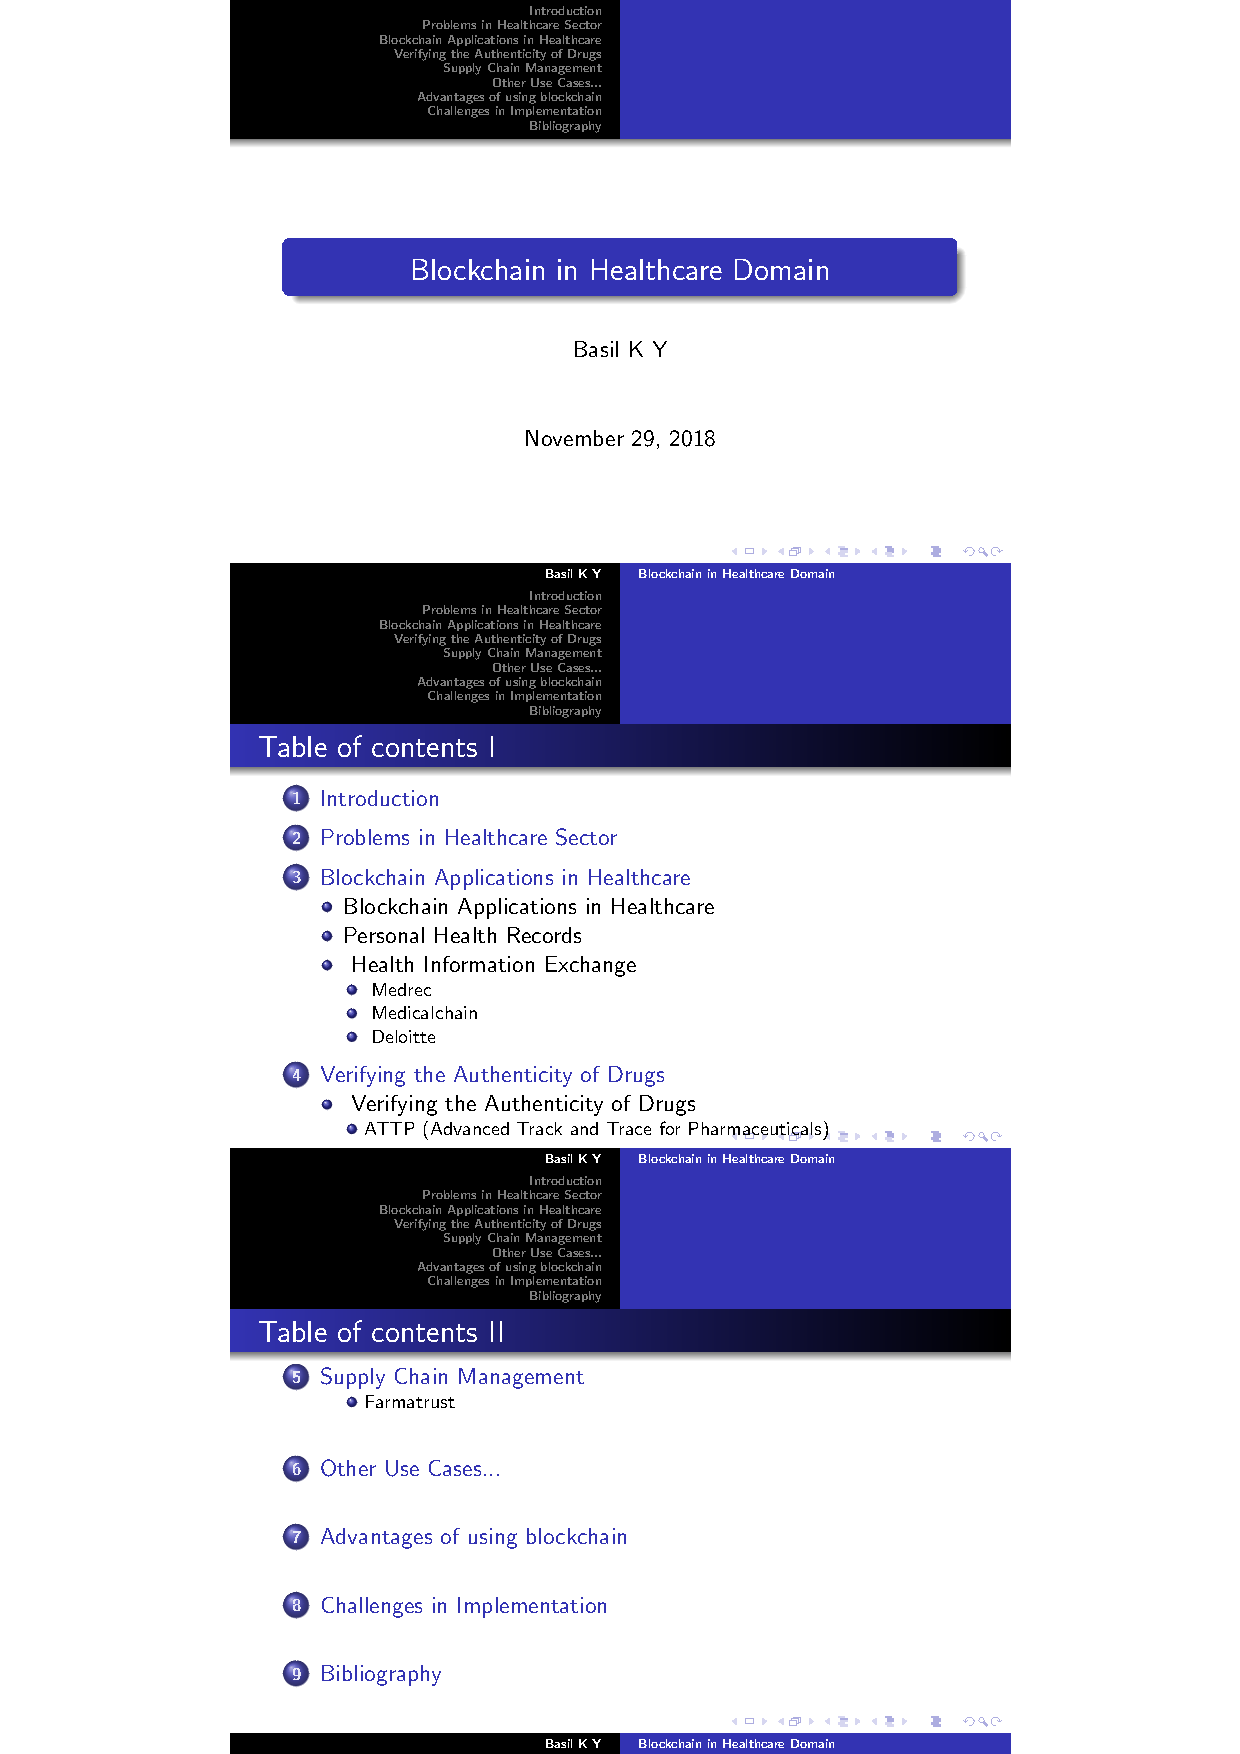
\includepdf[pages=-,offset=20 0,width=1.2\textwidth]{slide.pdf}

\chapter*{Viva }
\begin{enumerate}[label=\textbf{\arabic*})]
  \item \textbf{What are Merkle Trees?}
  \newline
  \newline
  Merkle trees are a fundamental part of blockchain technology. A merkle tree is a structure that allows for efficient and secure verification of content in a large body of data. This structure helps verify the consistency and content of the data. The Merkle Root summarizes all of the data in the related transactions, and is stored in the block header.
  \item \textbf{Why data on blockchain is immutable?}
  \newline
  \newline  
  If a miner tries to change a transaction from history, he will have to re-mine all the blocks from that block till the current block and this will have to be reflected in every copy of the ledger in the network. Miners will have to rebuild the merkle tree of the block in which the transaction is present and redo all the proof of work for that block.The computing power required to achieve this is enormous and probably only theoretical.
    \item \textbf{Is it possible to change data on blockchain if any correction is needed?}
    \newline
    \newline
    Blockchain is a series of records linked using the hashes of records, which provides immutability to the data on blockchain. Since data on blockchain is immutable, it can't be changed.But if any correction is needed on the existing data, we can add a new block stating the error in the previous blocks.The erroneous records will still exist in the blockchain network.
    
\end{enumerate}
\chapter*{\centering References}
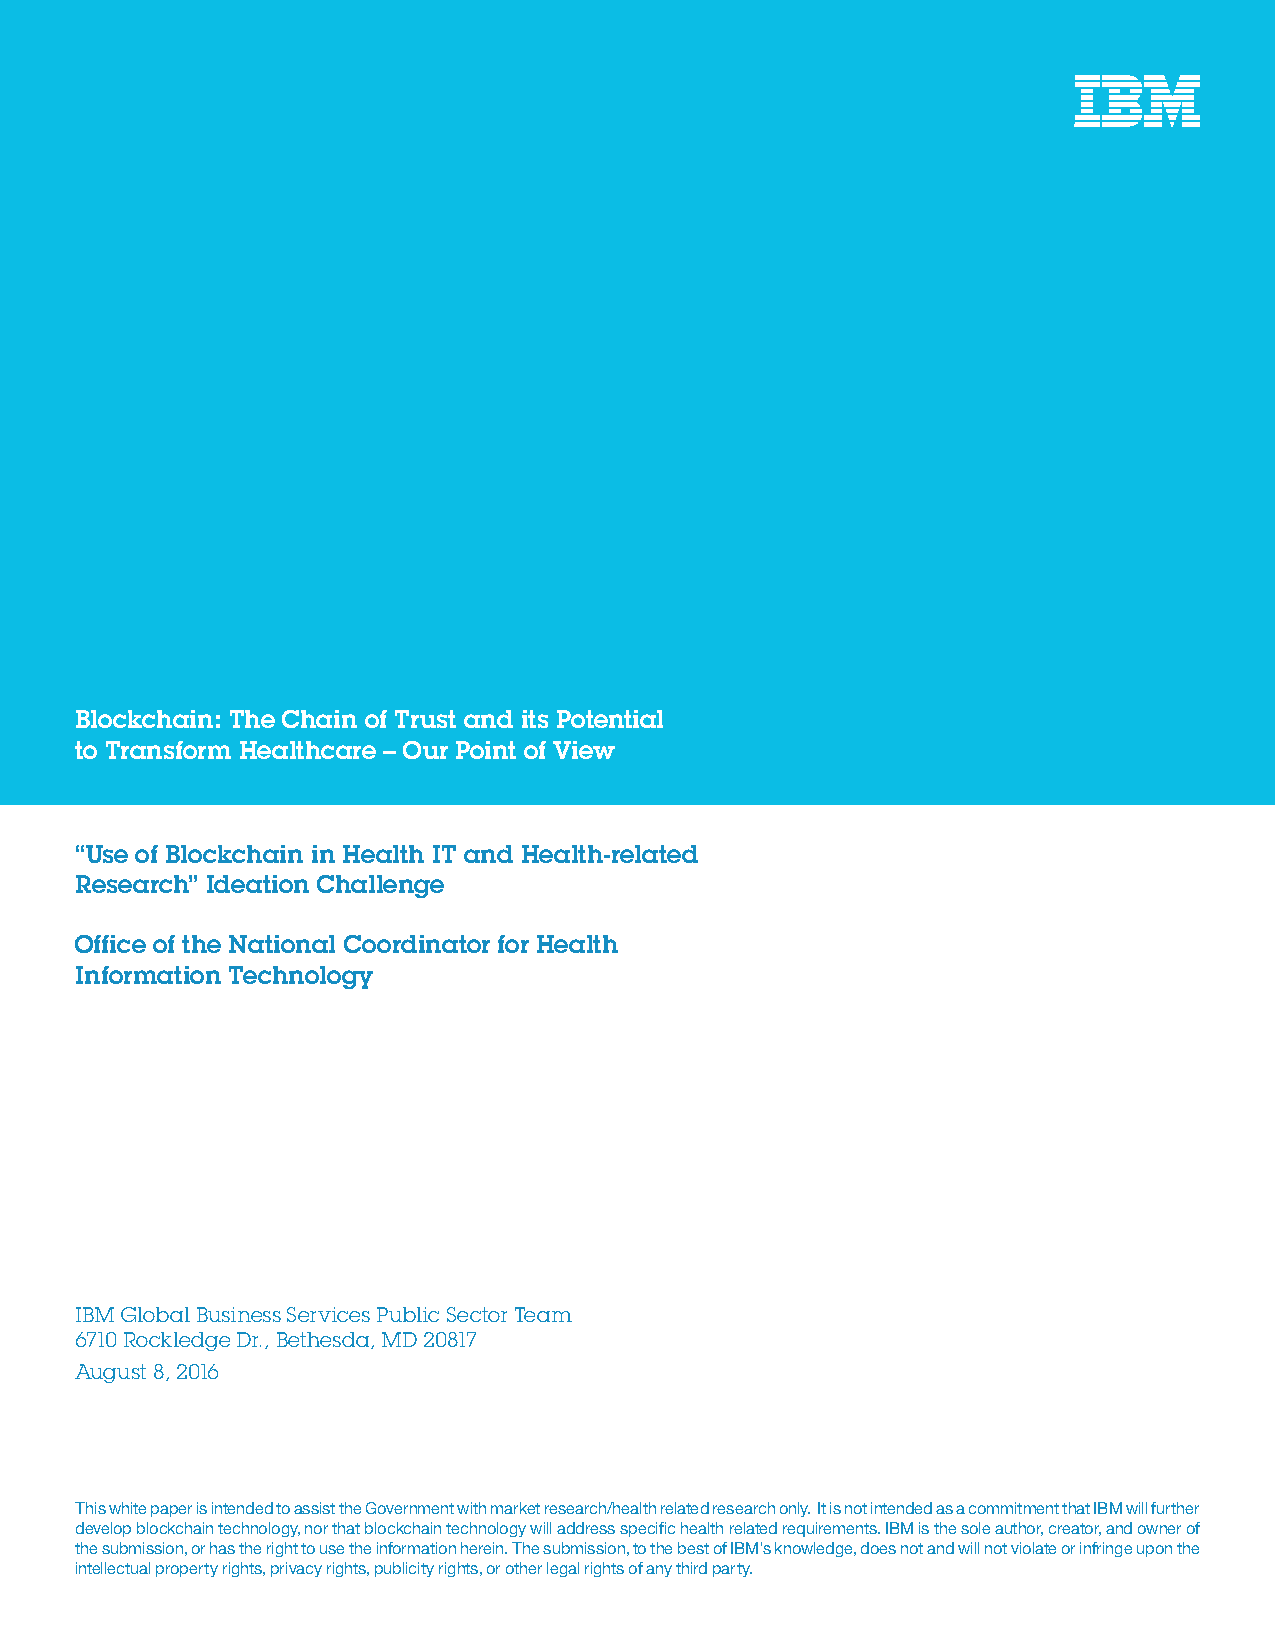
\includepdf[pages=1,offset=20 0,width=1.15\textwidth]{10.pdf}
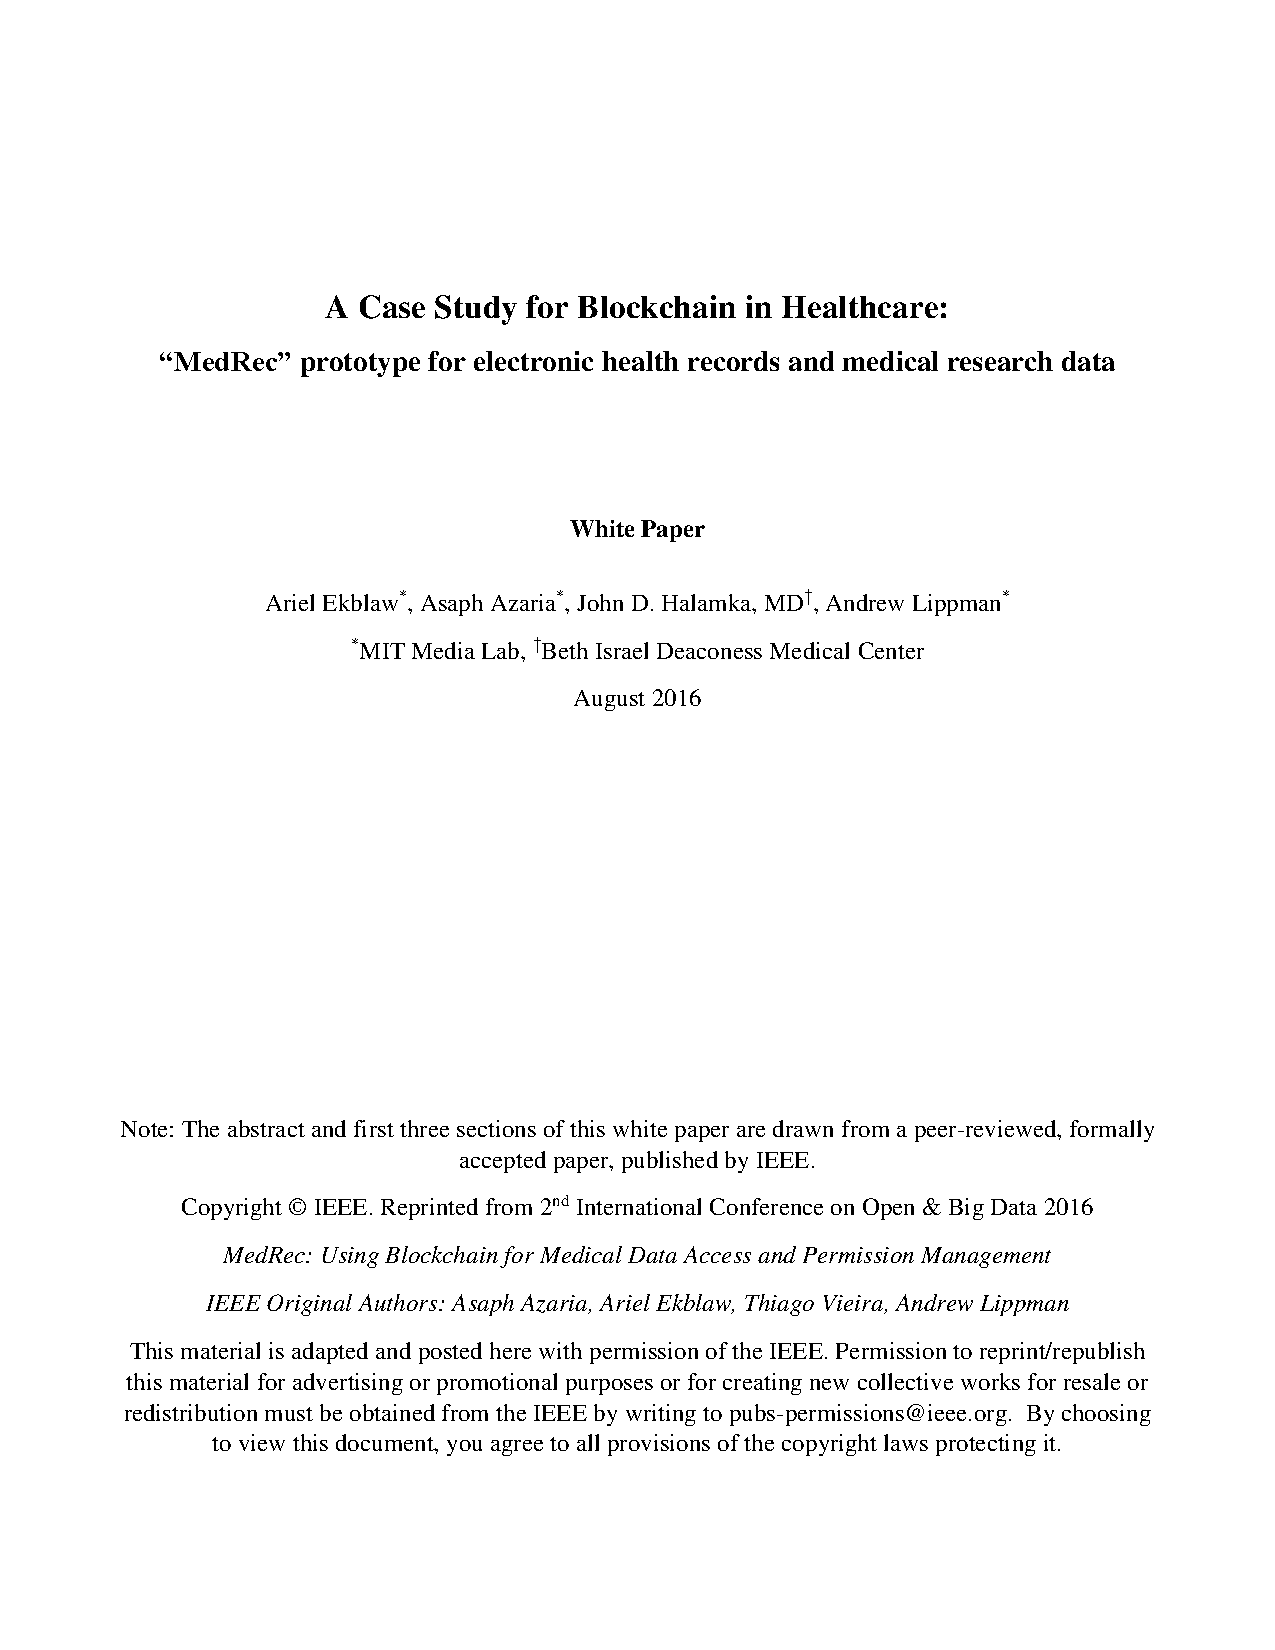
\includepdf[pages=1,offset=20 0,width=1.15\textwidth]{8.pdf}
\includepdf[pages=4,offset=20 0,width=1.15\textwidth]{4.pdf}
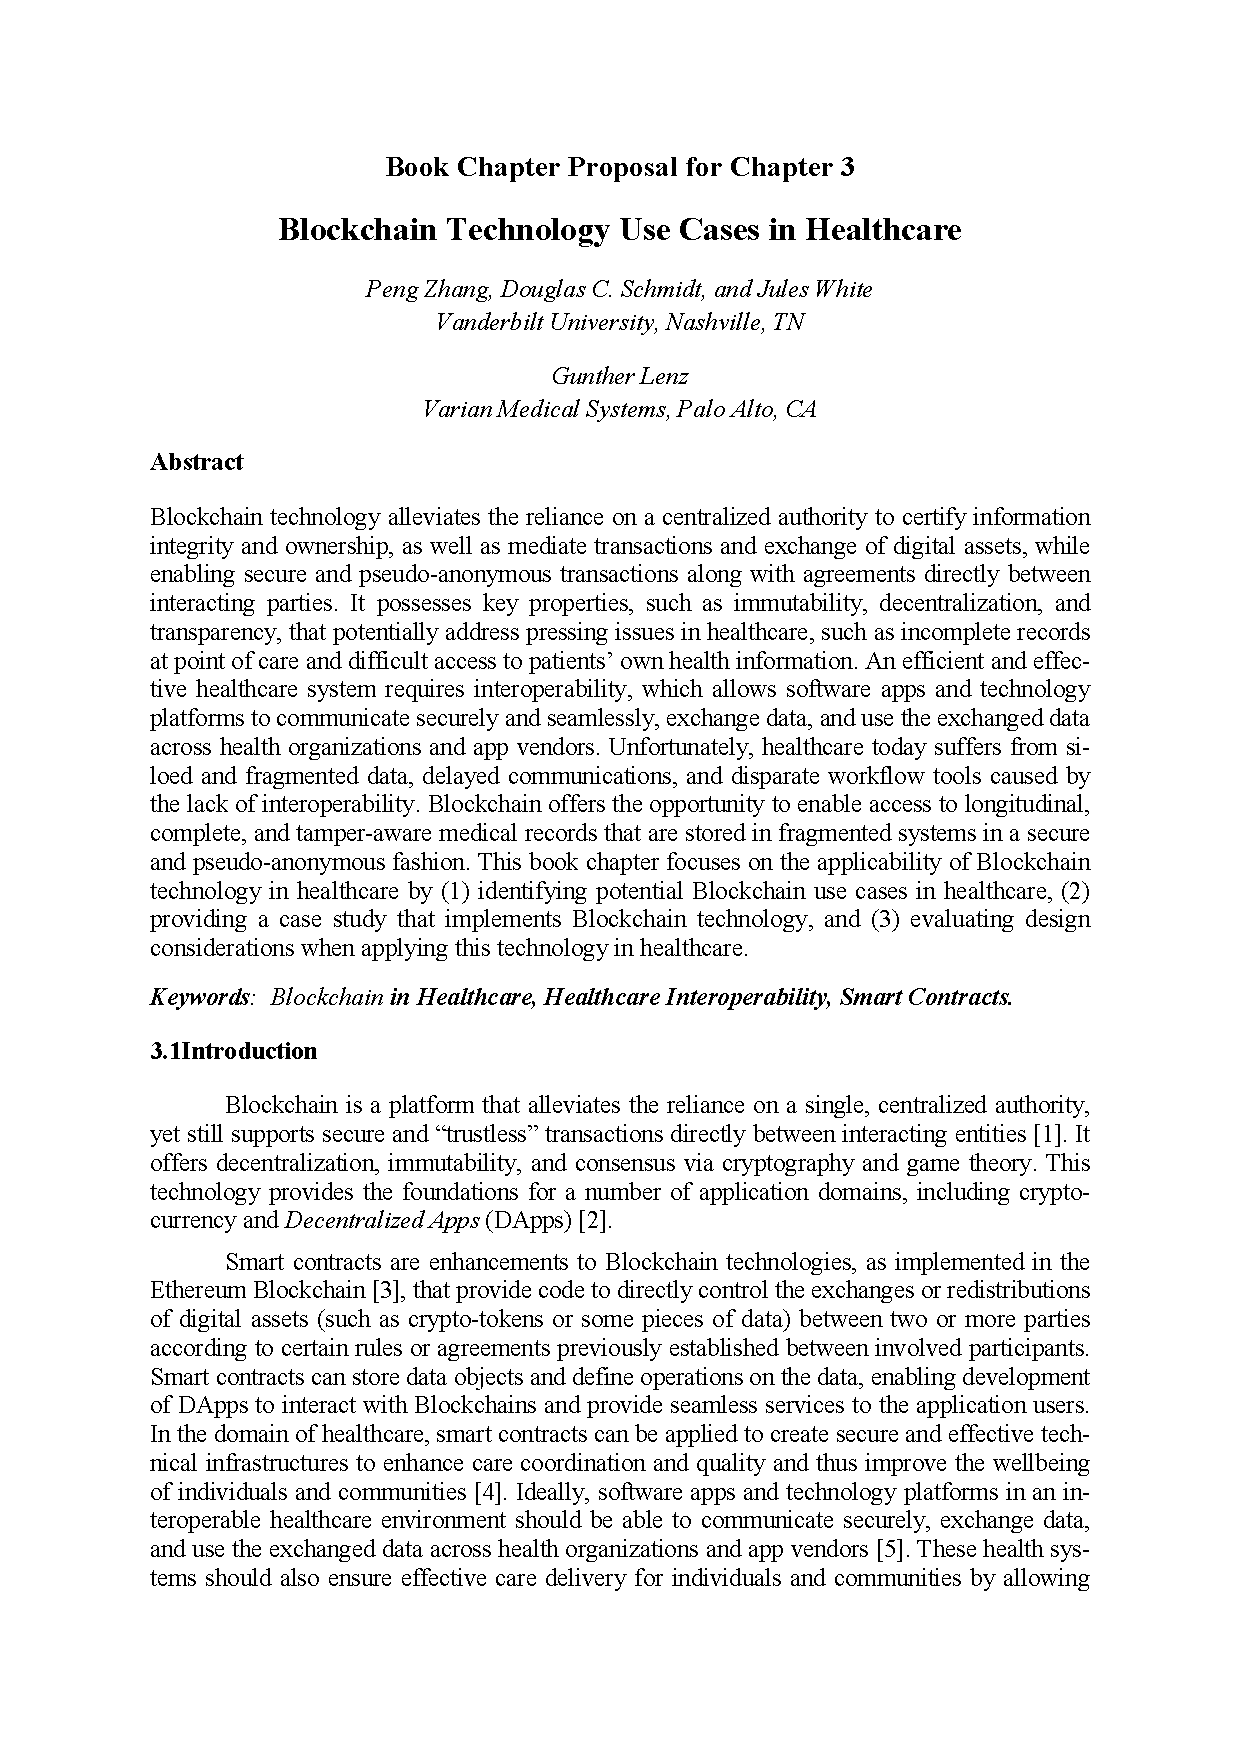
\includepdf[pages=1,offset=20 0,width=1.45\textwidth]{12.pdf}
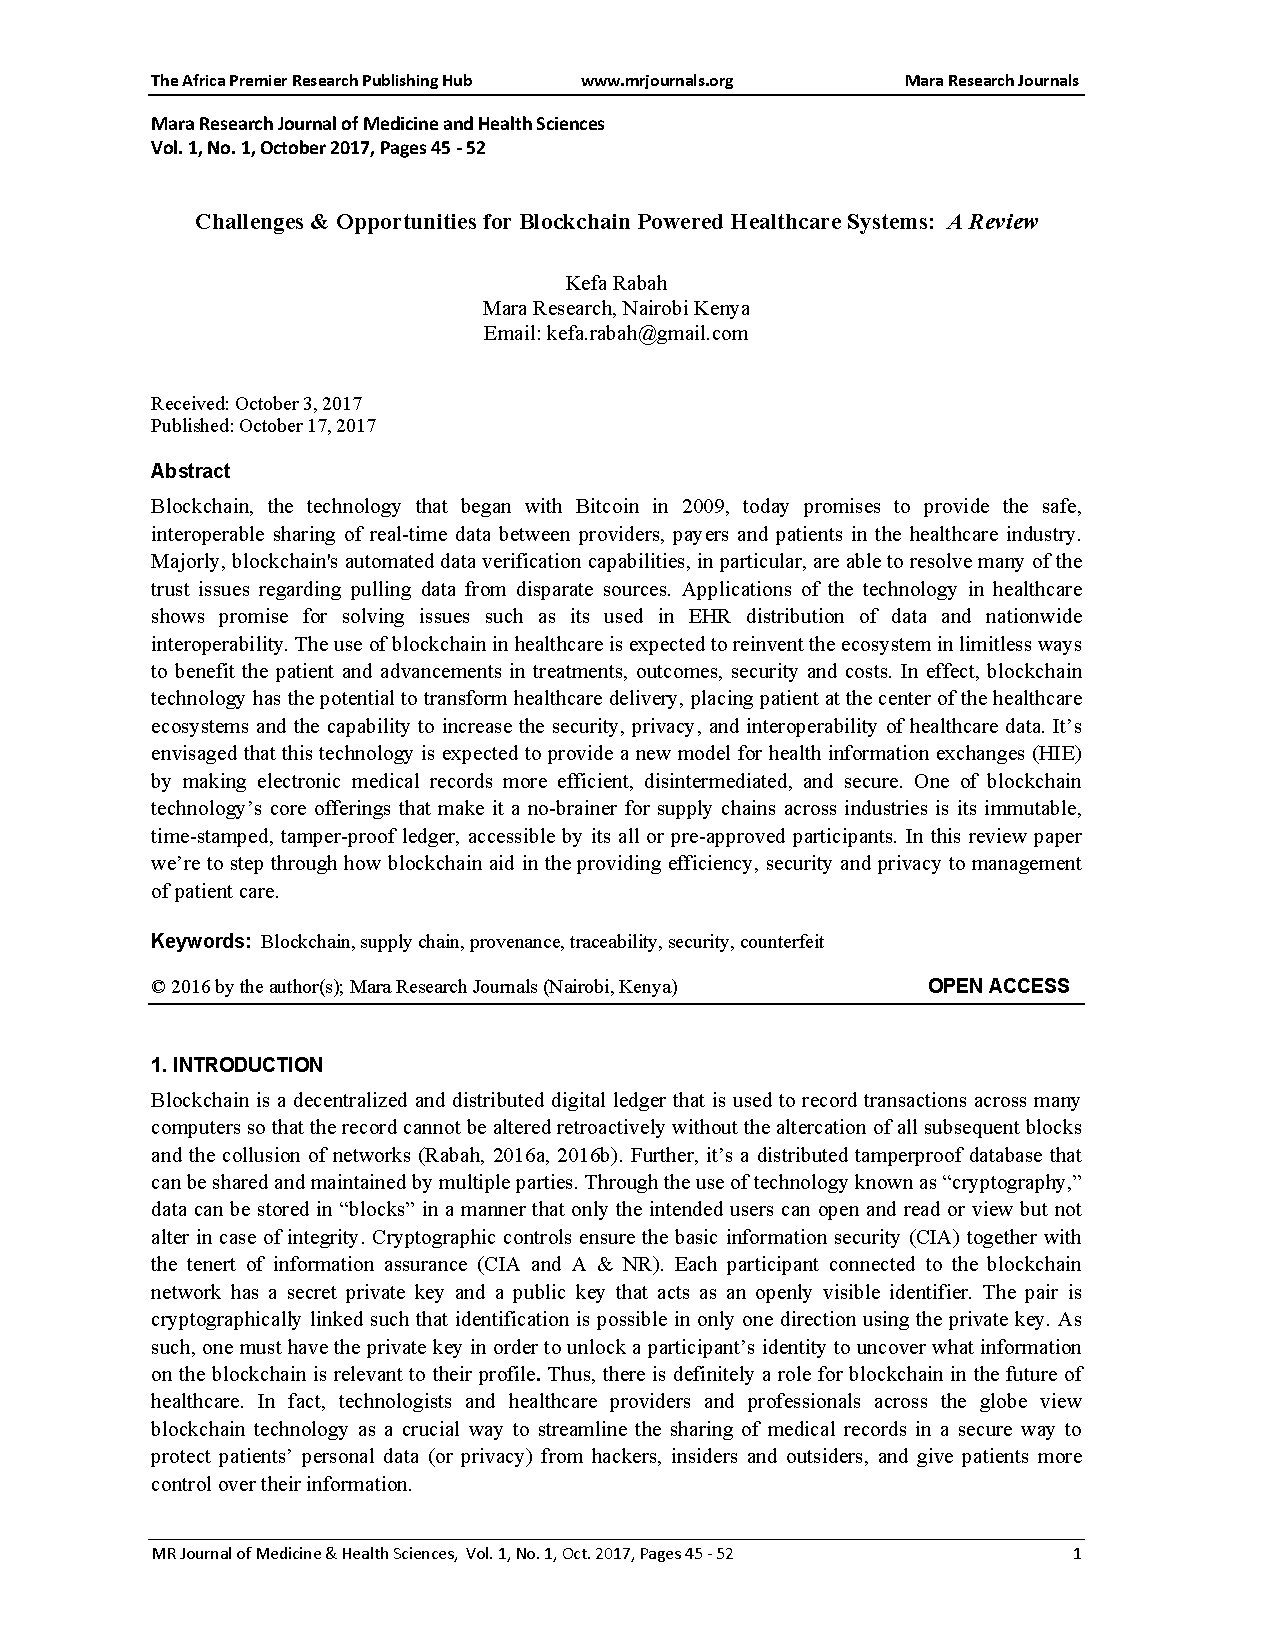
\includepdf[pages=1,offset=20 0,width=1.45\textwidth]{9.pdf}
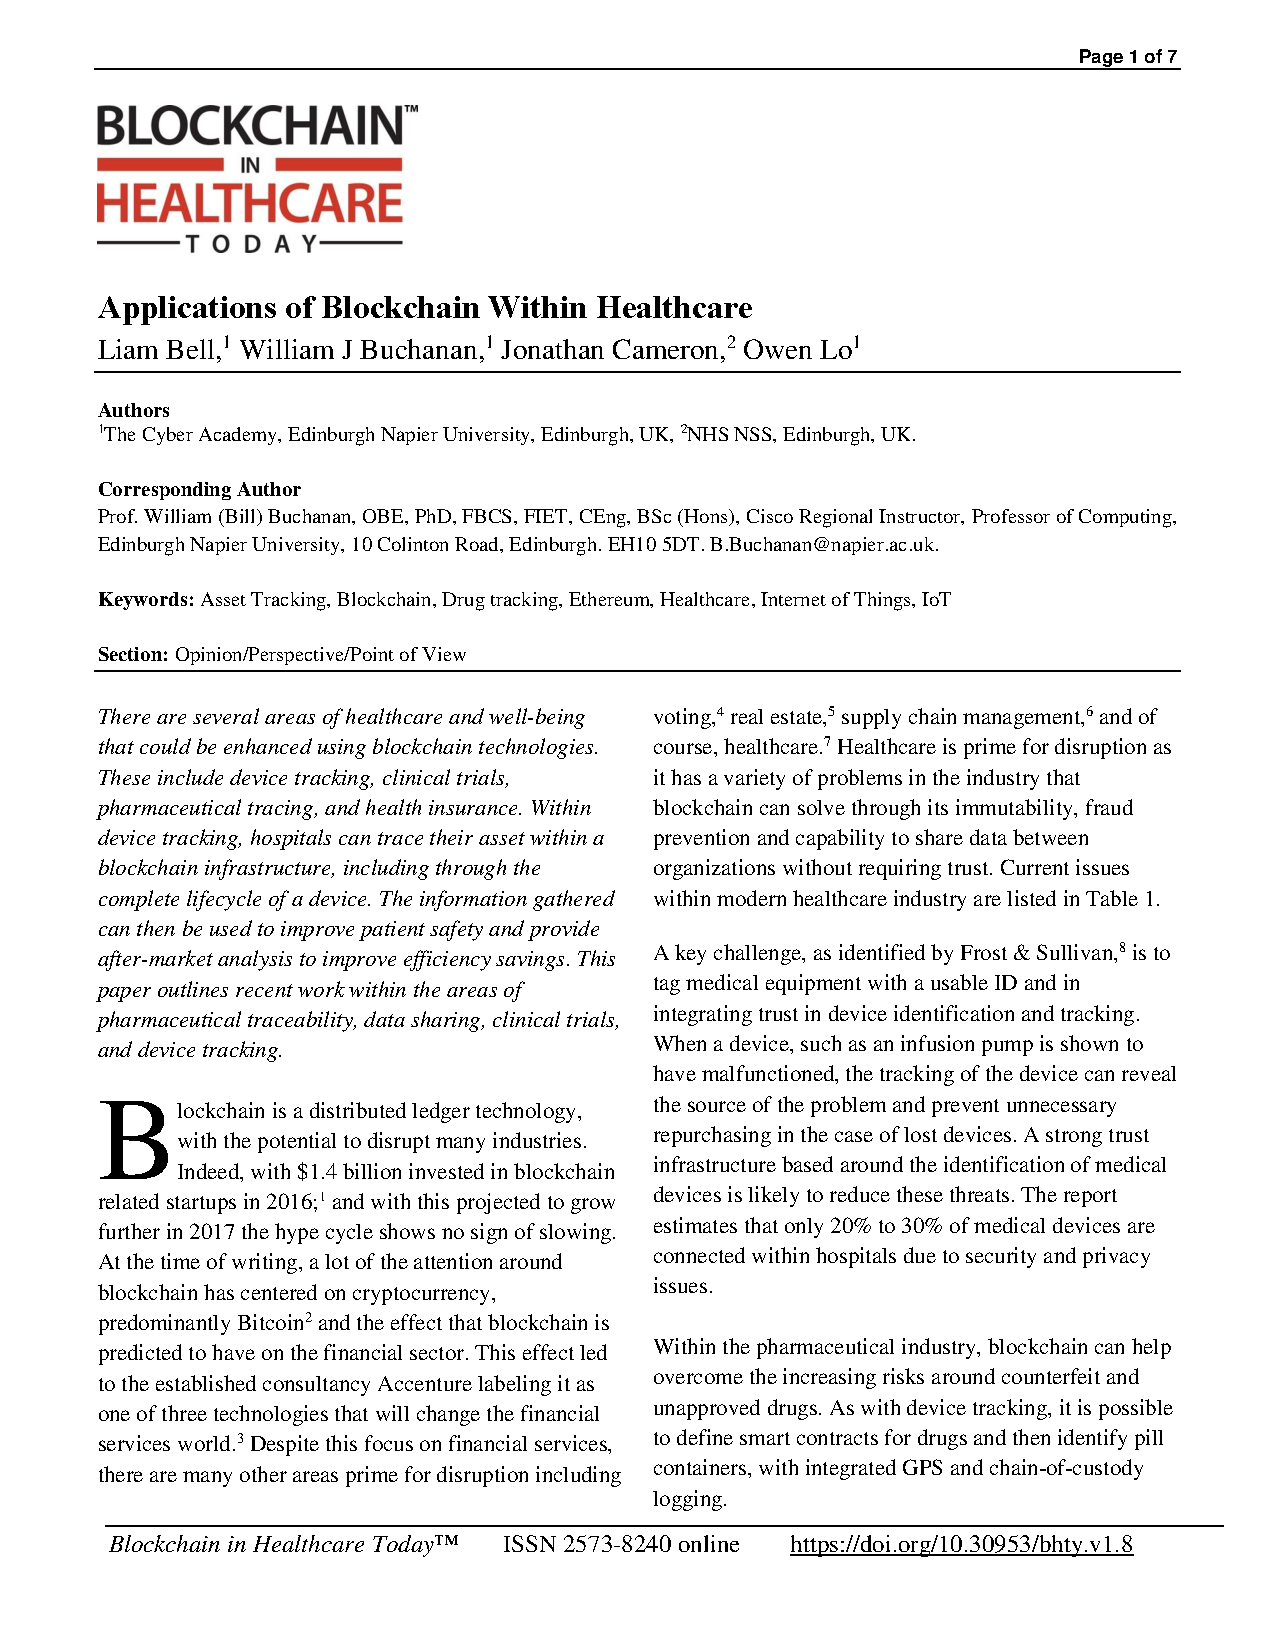
\includepdf[pages=1,offset=15 0,width=1.3\textwidth]{11.pdf}
\includepdf[pages=3,offset=15 0,width=1.3\textwidth]{3.pdf}
\end{appendices}
\end{document}